\subsection{Esercizio 3.7 - Hoff}

Posterior prediction: Consider a pilot study in which $n_1$ = 15 children enrolled in special education classes were randomly selected and tested for a certain type of learning disability. In the pilot study, $y_1$ = 2 children tested positive for the disability.

\begin{enumerate}[label=\alph*)]
    \item Using a uniform prior distribution, find the posterior distribution of $\theta$, the fraction of students in special education classes who have the disability. Find the posterior mean, mode and standard deviation of $\theta$, and plot the posterior density.
    \par Researchers would like to recruit students with the disability to participate in a long-term study, but first they need to make sure they can recruit enough students. Let $n_2 = 278$ be the number of children in special education classes in this particular school disctrict, and let $Y_2$ be the number of students with the disability.
    
    \item find $Pr(Y_2=y_2 | Y_1 = 2)$, the posterior predictive disctribution of $Y_2$, as follows:
    \begin{enumerate}[label=\roman*.]
        \item Discuss what assumptions are needed about the joint distribution of $(Y_1,Y_2)$ such that the following is true:
        \begin{align*}
            Pr(Y_2=y_2) = \int_0^1 Pr(Y_2=y_2|\theta)p(\theta|Y_1=2)\ d\theta 
        \end{align*}
        \item Now plug in the forms for $Pr(Y_2=y_2|\theta)$ and $p(\theta|Y_1=2)$ in the above integral.
        \item Figure out what the above integral must be by using the calculus result discussed in Section 3.1
    \end{enumerate}
    \item Plot the function $Pr(Y_2=y_2|Y_1=2)$ as a function of $y_2$. Obtain the mean and standard deviation of $Y_2$, given $Y_1$=2.
    \item The posterior mode and the MLE (maximum likelihood estimate; see Excercise 3.14) of $\theta$, based on data from the pilot study, are both $\hat{\theta} = 2/15$. Plot the distribution $Pr(Y_2=y_2|\theta=\hat{\theta})$, and find the mean and standard deviation of $Y_2$ give $\theta=\hat{\theta}$. Compare these results to the plots and calculations in c) and discuss any differences. Which distribution for $Y_2$ would you use to make prediction, and why?
\end{enumerate}

\textbf{Svolgimento}
\bigskip

a) Possiamo modellare lo studio trattato nel testo con una distribuzione binomiale ovvero

\begin{align*}
    P(\textbf{y}|\theta) = \theta^{y}(1-\theta)^{1-y}
\end{align*}

e come indicato dal testo useremo come prior una uniforme

\begin{align*}
    P(\theta)= \mathds{1}[0,1]^\theta
\end{align*}

Procediamo adesso al calcolo della \textit{a posteriori}.

\begin{align*}
    P(\theta|\textbf{y}) &= K  \times \mathcal{L}(\theta;\textbf{y})\times P(\theta)\\
    &= K \times \left(\prod_{i=1}^{15}\theta^{y_i}(1-\theta)^{1-y_i}\right)\times\mathds{1}[0,1]^\theta\\
    &\text{...avendo 2 ``successi'' e 13 ``insuccessi'' avremo...} \\
    &= K \times \theta^2(1-\theta)^{13} \times \mathds{1}[0,1]^\theta
\end{align*}

Per calcolare il valore $K$ e volendo trovare una distribuzione di probabilità propria, sappiamo che l'integrale di quest'ultima dovrà essere uguale a 1 nello spazio ammissibile di $\theta$, ovvero

\begin{align*}
   1 &= \int_0^1 K \times \theta^2(1-\theta)^{13} \times \mathds{1}[0,1]^\theta\ d\theta \\
    &= K \int_0^1  \theta^2(1-\theta)^{13}\ d\theta
\end{align*}

Si riconosce il kernel di una distribuzione Beta(3,14) e quindi si può moltiplicare e dividere per la sua costante di normalizzazione
\begin{align*}
    1 &= K \int_0^1  \theta^2(1-\theta)^{13} \frac{\Gamma(17)}{\Gamma(3)\Gamma(14)} \frac{\Gamma(3)\Gamma(14)}{\Gamma(17)}\ d\theta\\
    &= K \times \frac{\Gamma(3)\Gamma(14)}{\Gamma(17)} \underbrace{\int_0^1  \theta^2(1-\theta)^{13} \frac{\Gamma(17)}{\Gamma(3)\Gamma(14)}\ d\theta}_\text{=1}\\
    \frac{1}{K}&=\frac{\Gamma(3)\Gamma(14)}{\Gamma(17)}
\end{align*}

Si conclude quindi che

\begin{align*}
    P(\theta|\textbf{y}) &= \frac{\Gamma(17)}{\Gamma(3)\Gamma(14)} \theta^2(1-\theta)^{13} \\
    &\sim Beta(3,14)
\end{align*}

dalla quale si può facilmente calcolare valore medio, moda e standard deviation

\begin{align*}
    E(\theta|\textbf{y}) &= \frac{\alpha}{\alpha + \beta} = \frac{3}{17}\\
    Moda(\theta|\textbf{y}) &= \frac{\alpha-1}{\alpha + \beta-2} = \frac{2}{15}\\
    Var(\theta|\textbf{y}) &= \frac{\alpha\beta}{(\alpha + \beta)^2(\alpha + \beta + 1)} = \frac{42}{17^2\times 18} \approx 8*10^{-3}
\end{align*}

In Figura \ref{fig:beta} si mostra la distribuzione appena calcolata

\begin{figure}[!ht]
\centering
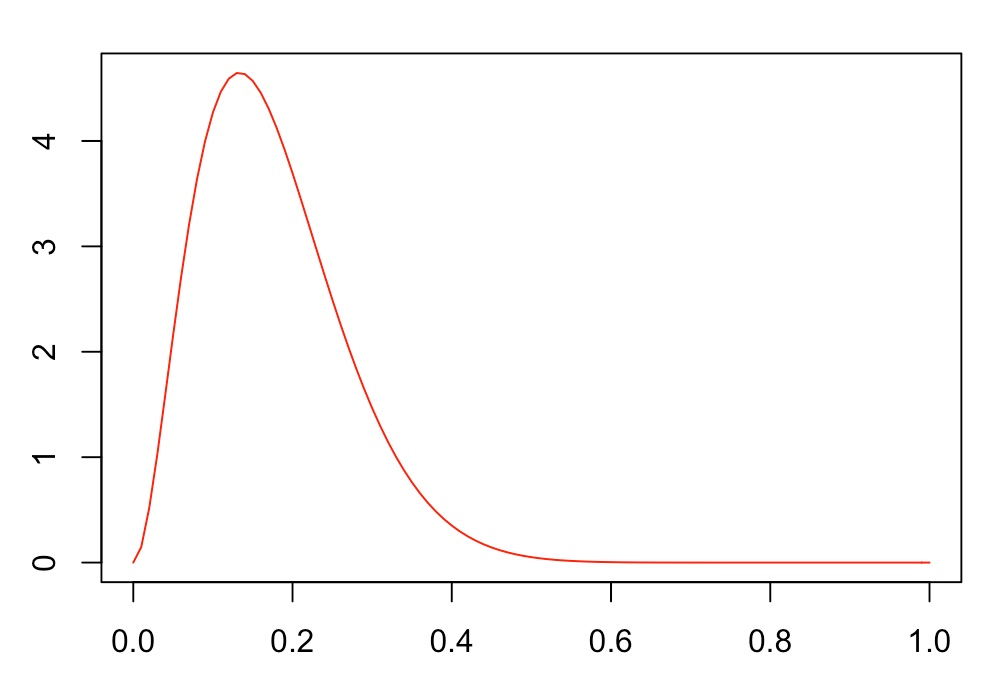
\includegraphics[width=0.6\textwidth]{img/esercizio3-07-Beta314}
\caption{una Beta(3,14)}
\label{fig:beta}
\end{figure}

b) Affinchè
\begin{equation} \label{eq:1}
    Pr(Y_2=y_2) = \int_0^1 Pr(Y_2=y_2|\theta)p(\theta|Y_1=2) \ d\theta
\end{equation}
dobbiamo innanzitutto assumere che la distribuzione predittiva non dipenda da quantità 
incognite ma dipenda dai dati osservati (altrimenti sarebbe inutilizzabile ai fini 
predittivi), ma che il valore predetto sia indipendente dai dati osservati dato $\theta$, ovvero 
\begin{align*}
    Y_2 \perp\!\!\!\perp Y_1 | \theta \\
    (\text{ma non } Y_2 \perp\!\!\!\perp Y_1)
\end{align*}

Con queste assunzioni otterremo che $Pr(Y_2|\theta,Y_1) = Pr(Y_2|\theta)$ e quindi l'equazione (\ref{eq:1}) risulterà valida. \\
Considerando le assunzioni del testo e svolgendo i calcoli avremo quanto segue:

\begin{align*}
     Pr(Y_2=y_2) &= \int_0^1 Pr(Y_2=y_2|\theta)p(\theta|Y_1=2) \ d\theta\\
     &= \int_0^1 \binom{278}{y_2}\theta^{y_2}(1-\theta)^{278-y_2} \frac{\Gamma(17)}{\Gamma(3)\Gamma(14)} \theta^2(1-\theta)^{13}\ d\theta\\
      &= \binom{278}{y_2} \frac{\Gamma(17)}{\Gamma(3)\Gamma(14)} \int_0^1 \theta^{y_2 + 2}(1-\theta)^{291-y_2}\ d\theta
\end{align*}

Si riconosce nell'integrale il kernel di una Beta($y_2+3,292-y_2$) e quindi utilizzando 
la stessa tecnica vista al punto precedente avremo

\begin{align*}
     Pr(Y_2=y_2) &= \binom{278}{y_2} \frac{\Gamma(17)}{\Gamma(3)\Gamma(14)} \frac{\Gamma(y_2+3)\Gamma(292-y_2)}{\Gamma(295)}\\
     &=  \frac{\Gamma(3+14)}{\Gamma(3)\Gamma(14)\Gamma(3+14+278)}\binom{278}{y_2} \Gamma(3+y_2)\Gamma(14+278-y_2)
\end{align*}

ovvero una \textbf{Beta-Binomiale(3, 14, 278)} 
(rappresentata in Figura \ref{fig:betaBinomiale}) dalla quale si può 
facilmente calcolare media e standard deviation:

\begin{align*}
    E(Y_2|Y_1=2) &= n\frac{\alpha}{\alpha + \beta} = 278\frac{3}{17} \approx 49,06\\
    Var(Y_2|Y_1=2) &= \frac{n\alpha\beta}{(\alpha + \beta)^2}\times\frac{(\alpha + \beta + n)}{(\alpha + \beta + 1)} = \frac{278\times3\times14}{17^2} \times\frac{295}{18} \approx 662,13
\end{align*}


\begin{figure}[!ht]
\centering
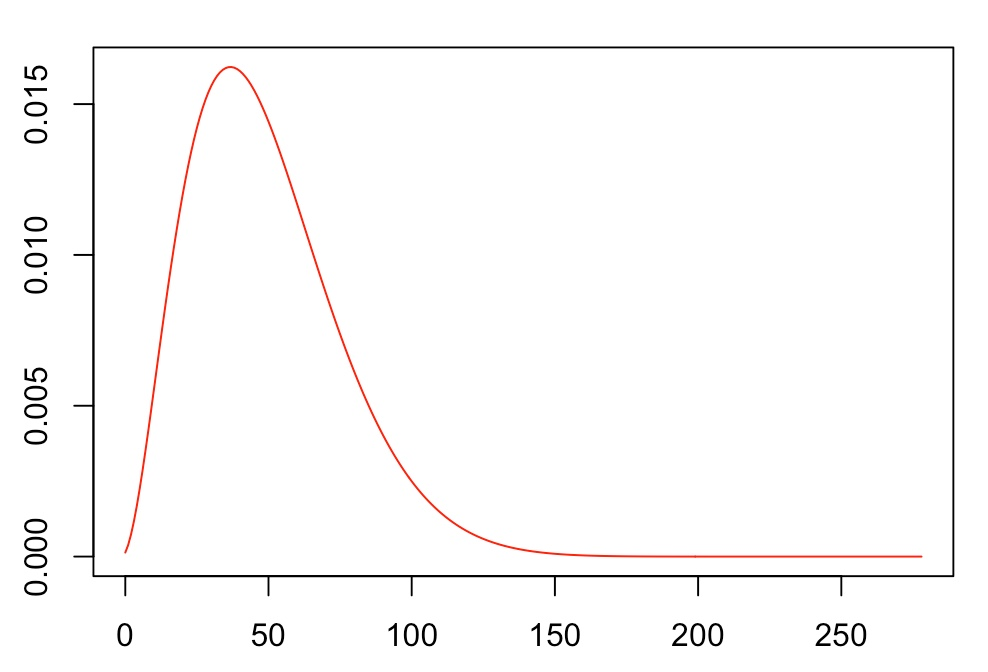
\includegraphics[width=0.6\textwidth]{img/esercizio3-07-BetaBinomiale}
\caption{Beta-Binomiale(3, 14, 278)}
\label{fig:betaBinomiale}
\end{figure}

Supponendo che la moda a posteriori e la MLE di $\theta$ siano entrambe $\hat{\theta}$ = 2/15 allora avremo 

\begin{align*}
    P\left(Y_2=y_2|\theta=\frac{2}{15}\right) &= \binom{278}{y_2}\left(\frac{2}{15}\right)^{y_2}\left(1-\frac{2}{15}\right)^{278-y_2} \\
    &\sim Binomiale\left(\frac{2}{15},278\right)
\end{align*}

Otteniamo quindi una distribuzione binomiale (rappresentata nella parte destra di Figura \ref{fig:Binomiale}) con relative media e standard deviation:

\begin{align*}
    E\left(Y_2=y_2|\theta=\frac{2}{15}\right) &= n\theta = 278\times\frac{2}{15} \approx 37,07\\
    Var\left(Y_2=y_2|\theta=\frac{2}{15}\right)  &= n\theta (1-\theta) = 278\times\frac{2}{15} \times \frac{13}{15} \approx 32,12
\end{align*}


\begin{figure}[!ht]
\begin{minipage}[b]{0.47\textwidth}
\centering
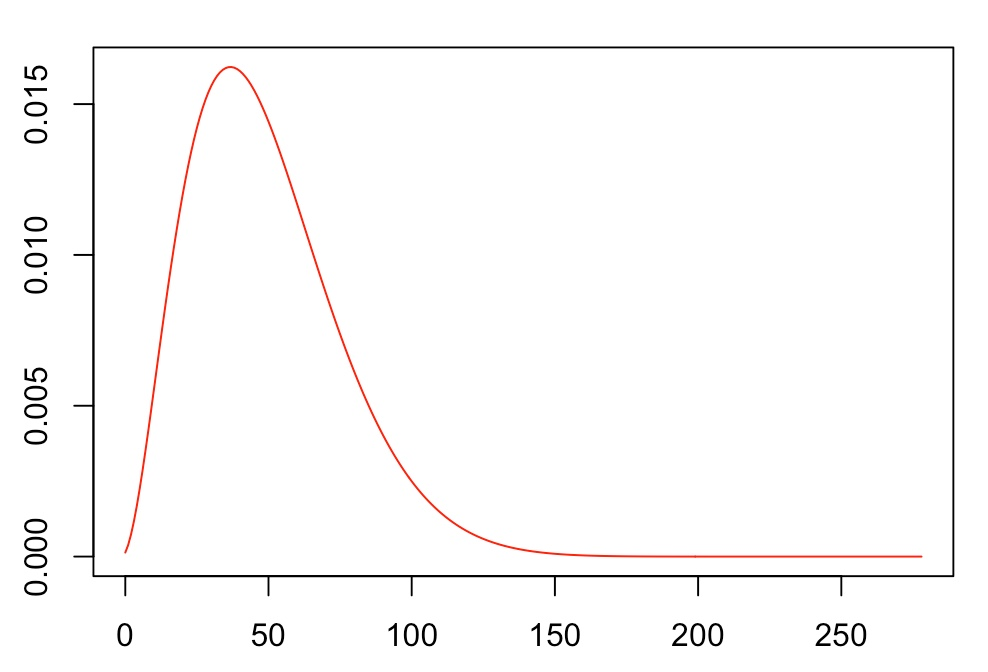
\includegraphics[width=\textwidth]{img/esercizio3-07-BetaBinomiale}
\end{minipage}
\hfill
\begin{minipage}[b]{0.47\textwidth}
\centering
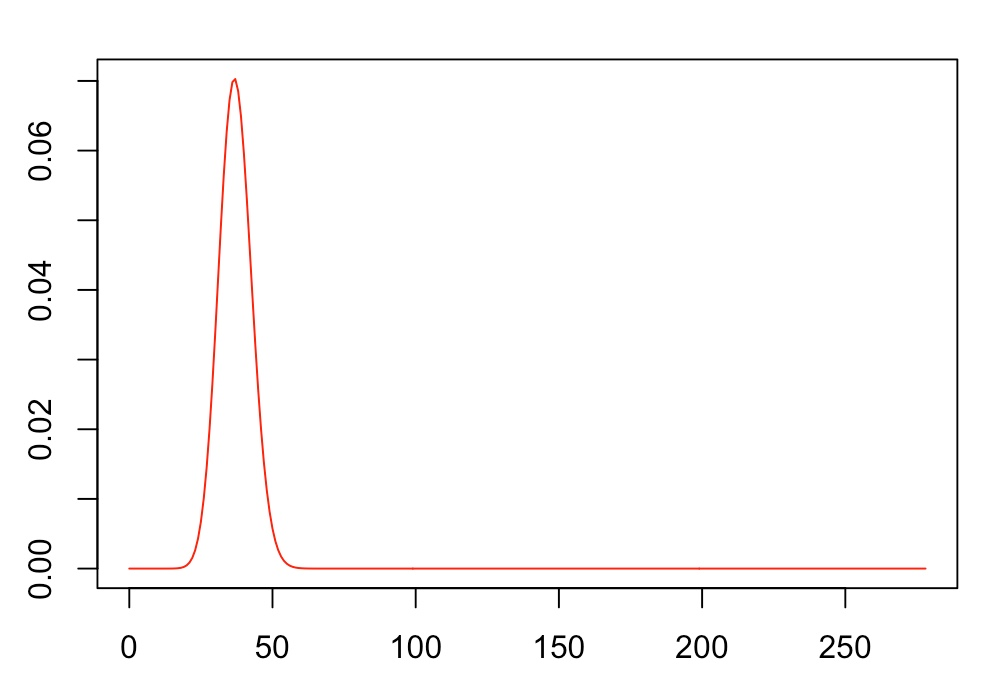
\includegraphics[width=\textwidth]{img/esercizio3-07-Binomiale}
\end{minipage}
\caption{Una Betabinomiale(3, 14, 278) (a sinistra) e una Binomiale(2/15, 278) (a destra) a confronto}.
\label{fig:Binomiale}
\end{figure}

Risulta evidente come media e moda delle due distribuzioni siano piuttosto simili a 
differenza della varianza che risulta notevolmente più bassa nella Binomiale. 
Questo risultato piuttosto intuitivo è dovuto all'aver fissato il parametro $\theta$ 
nel secondo metodo, che ha come effetto una drastica riduzione dell'intervallo di 
confidenza rispetto alla media della nostra predizione. 

Concludendo, per la  predizione di $Y_2$, preferiremo utilizzare quest'ultima variante 
ovvero assegnare a $\theta$ la MLE, che nonostante sia in leggera contrad\-dizione con 
la definizione bayesiana di \textit{a priori} (come vedremo nell'esercizio 3.14) ha 
come effetto una notevole riduzione della variabilità della nostra predizione.